\appendix

\chapter{Список публікацій здобувача за темою дисертації}
\vspace*{-1\baselineskip}
\textit{\textbf{Наукові праці, в яких опубліковані основні наукові результати дисертації:}}
\medskip

\begin{enumerate}
    \item Ніколаєв, Андрій Д. та Анісімов, Анатолій В. \textit{Нейромережеві методи відбору та генерації синтетичних варіацій комбінаторних задач}. Кібернетика та системний аналіз. 2025, том 61, випуск 3, с.22-32. DOI: \url{https://doi.org/10.34229/KCA2522-9664.25.3.3}.
    \item Ніколаєв, Андрій. \textit{Нейромережеві методи формалізації математичних текстів}. Herald of Khmelnytskyi National University. Technical sciences, 345.6(2), 2024, с. 50—55. DOI: \url{https://doi.org/10.31891/2307-5732-2024-345-6-6}.
    \item Nikolaiev, Andrii D. та Derevianchenko, Oleksandr V. \textit{Comparison of Problem-solving Performance Across Mathematical Domains With Large Language Models}. Shtuchnyy intelekt, 2024, с. 96—104. \url{https://doi.org/10.15407/jai2024.04.096}.
    \item Власенко, О.В., Картавих, В.Ю., Ніколаєв, А.Д., Горбенко, В.І. \textit{Методика визначення опорної матриці моніторингу домена управління інформаційної мережі спеціального призначення}. Системи і технології зв’язку, інформатизації та кібербезпеки. Збірник наукових праць ВІТІ, випуск 4, 2019, с. 46—57.
\end{enumerate}

\medskip
\textit{\textbf{Наукові праці, які засвідчують апробацію матеріалів дисертації:}}
\medskip

\begin{enumerate}
    \item \textit{Introducing constraints in combinatorial problems: A case study with LLaMA 3.1}. -- 11th International Scientific Conference "Information Technology and Implementation (IT\&I-2024 Satellite)". Taras Shevchenko National University of Kyiv, 2024.
    \item \textit{AI in education: Application of LLMs for learning mathematics.} -- Ukrainian Cambridge: New Research by Displaced Scholars from Ukraine. University of Cambridge, 2023.
    \item Nikolaiev, Andrii D. and Anisimov, Anatoliy V. \textit{Mathematical word problem solution evaluation via data preprocessing approach}. 8th International Scientific Conference "Information Technology and Implementation (IT\&I-2021)", Vol. 3132, 2022, p. 94—103. \url{https://ceur-ws.org/Vol-3132/Paper_9.pdf} %\url{https://www.scopus.com/inward/record.uri?eid=2-s2.0-85129578190&partnerID=40&md5=63f41d66fe66b0b9088484ef474dcd4e}
    \item \textit{Implementation of Artificial Intelligence Module for Educational Purposes}. -- 7th International Scientific Conference "Information Technology and Interactions (IT\&I-2020 Satellite)". Taras Shevchenko National University of Kyiv, 2020.
\end{enumerate}

\medskip
\textit{\textbf{Наукові праці, які додатково відображають наукові результати дисертації:}}
\medskip
\begin{enumerate}
    \item Nikolaiev, Andrii, Stathopoulos, Yiannos та Teufel, Simone. \textit{Can language models rival mathematics students? Evaluating mathematical reasoning through textual manipulation and human experiments}. arXiv preprint, 2024. \url{https://arxiv.org/abs/2412.11908}.
\end{enumerate}

\chapter{Опис та доступи до протестованих моделей}
\label{sec:models-tested-links}
\vspace*{-1\baselineskip}
Детальні описи відкритих моделей (квантованих версій) та моделей від OpenAI доступні за наступними посиланнями:
\begin{enumerate}
    \item \textbf{LLaMA-2-7B-Chat}:\\
    \url{https://huggingface.co/TheBloke/Llama-2-7B-Chat-GGUF}.
    \item \textbf{LLaMA-2-13B-Chat}:\\
    \url{https://huggingface.co/TheBloke/Llama-2-13B-chat-GGUF}.
    \item \textbf{LLaMA-2-70B-Chat}:\\
    \url{https://huggingface.co/TheBloke/Llama-2-70B-Chat-GGUF}.
    \item \textbf{LLaMA-3.1-8B-Instruct}: \\
    \url{https://huggingface.co/QuantFactory/Meta-Llama-3.1-8B-Instruct-GGUF}.
    \item \textbf{LLaMA-3.1-70B-Instruct}:\\
    \url{https://huggingface.co/bartowski/Meta-Llama-3.1-70B-Instruct-GGUF}.
    \item \textbf{LLaMA-3.1-405B-Instruct}: (доступна через API)\\
    \url{https://build.nvidia.com/meta/llama-3_1-405b-instruct/modelcard}. 

    \item \textbf{Mixtral-8x7B}:\\
    \url{https://huggingface.co/TheBloke/Mixtral-8x7B-v0.1-GGUF}.
    \item \textbf{Mixtral-8x7B-Instruct}:\\
    \url{https://huggingface.co/TheBloke/Mixtral-8x7B-Instruct-v0.1-GGUF}.
    \item \textbf{Mathstral-7B}: \\
    \url{https://huggingface.co/QuantFactory/mathstral-7B-v0.1-GGUF}.

    \item \textbf{Qwen2-7B-Instruct}: \\
    \url{https://huggingface.co/QuantFactory/Qwen2-7B-Instruct-GGUF}.
    \item \textbf{Qwen2-Math-7B}: \\
    \url{https://huggingface.co/QuantFactory/Qwen2-Math-7B-GGUF}.
    \item \textbf{Qwen2.5-Math-7B}: \\
    \url{https://huggingface.co/QuantFactory/Qwen2.5-Math-7B-GGUF}.
    
    \item \textbf{GPT-4-Turbo}: (доступна через API)\\ 
    \url{https://platform.openai.com/docs/models/#gpt-4-turbo-and-gpt-4}.
    \item \textbf{GPT-4o-mini}: (доступна через API)\\
    \url{https://platform.openai.com/docs/models/gpt-4o-mini#gpt-4o-mini}.
\end{enumerate}

\chapter{Повні результати учасників експерименту}
\label{sec:humans-results-detailed}
\vspace*{-1\baselineskip}

На рис.~\ref{fig:human_results_detailed} можна бачити детальні результати роботи учасників у розв'язанні задач набору Combi-Puzzles.

Результати включають усіх 35 учасників, результати учасників ранжовані від найкращого до найгіршого у кожній з груп. Для формування загальних результатів, обиралися 5 ``експертів'' у кожній з груп (25 учасників разом) згідно постановки експерименту.

``0'' свідчить про те, що відповідь учасника була неправильною, ``1'' -- правильною, мінус -- учасник не передав відповідь на задачу (еквівалентно ``0'').

\begin{figure}
    \centering
    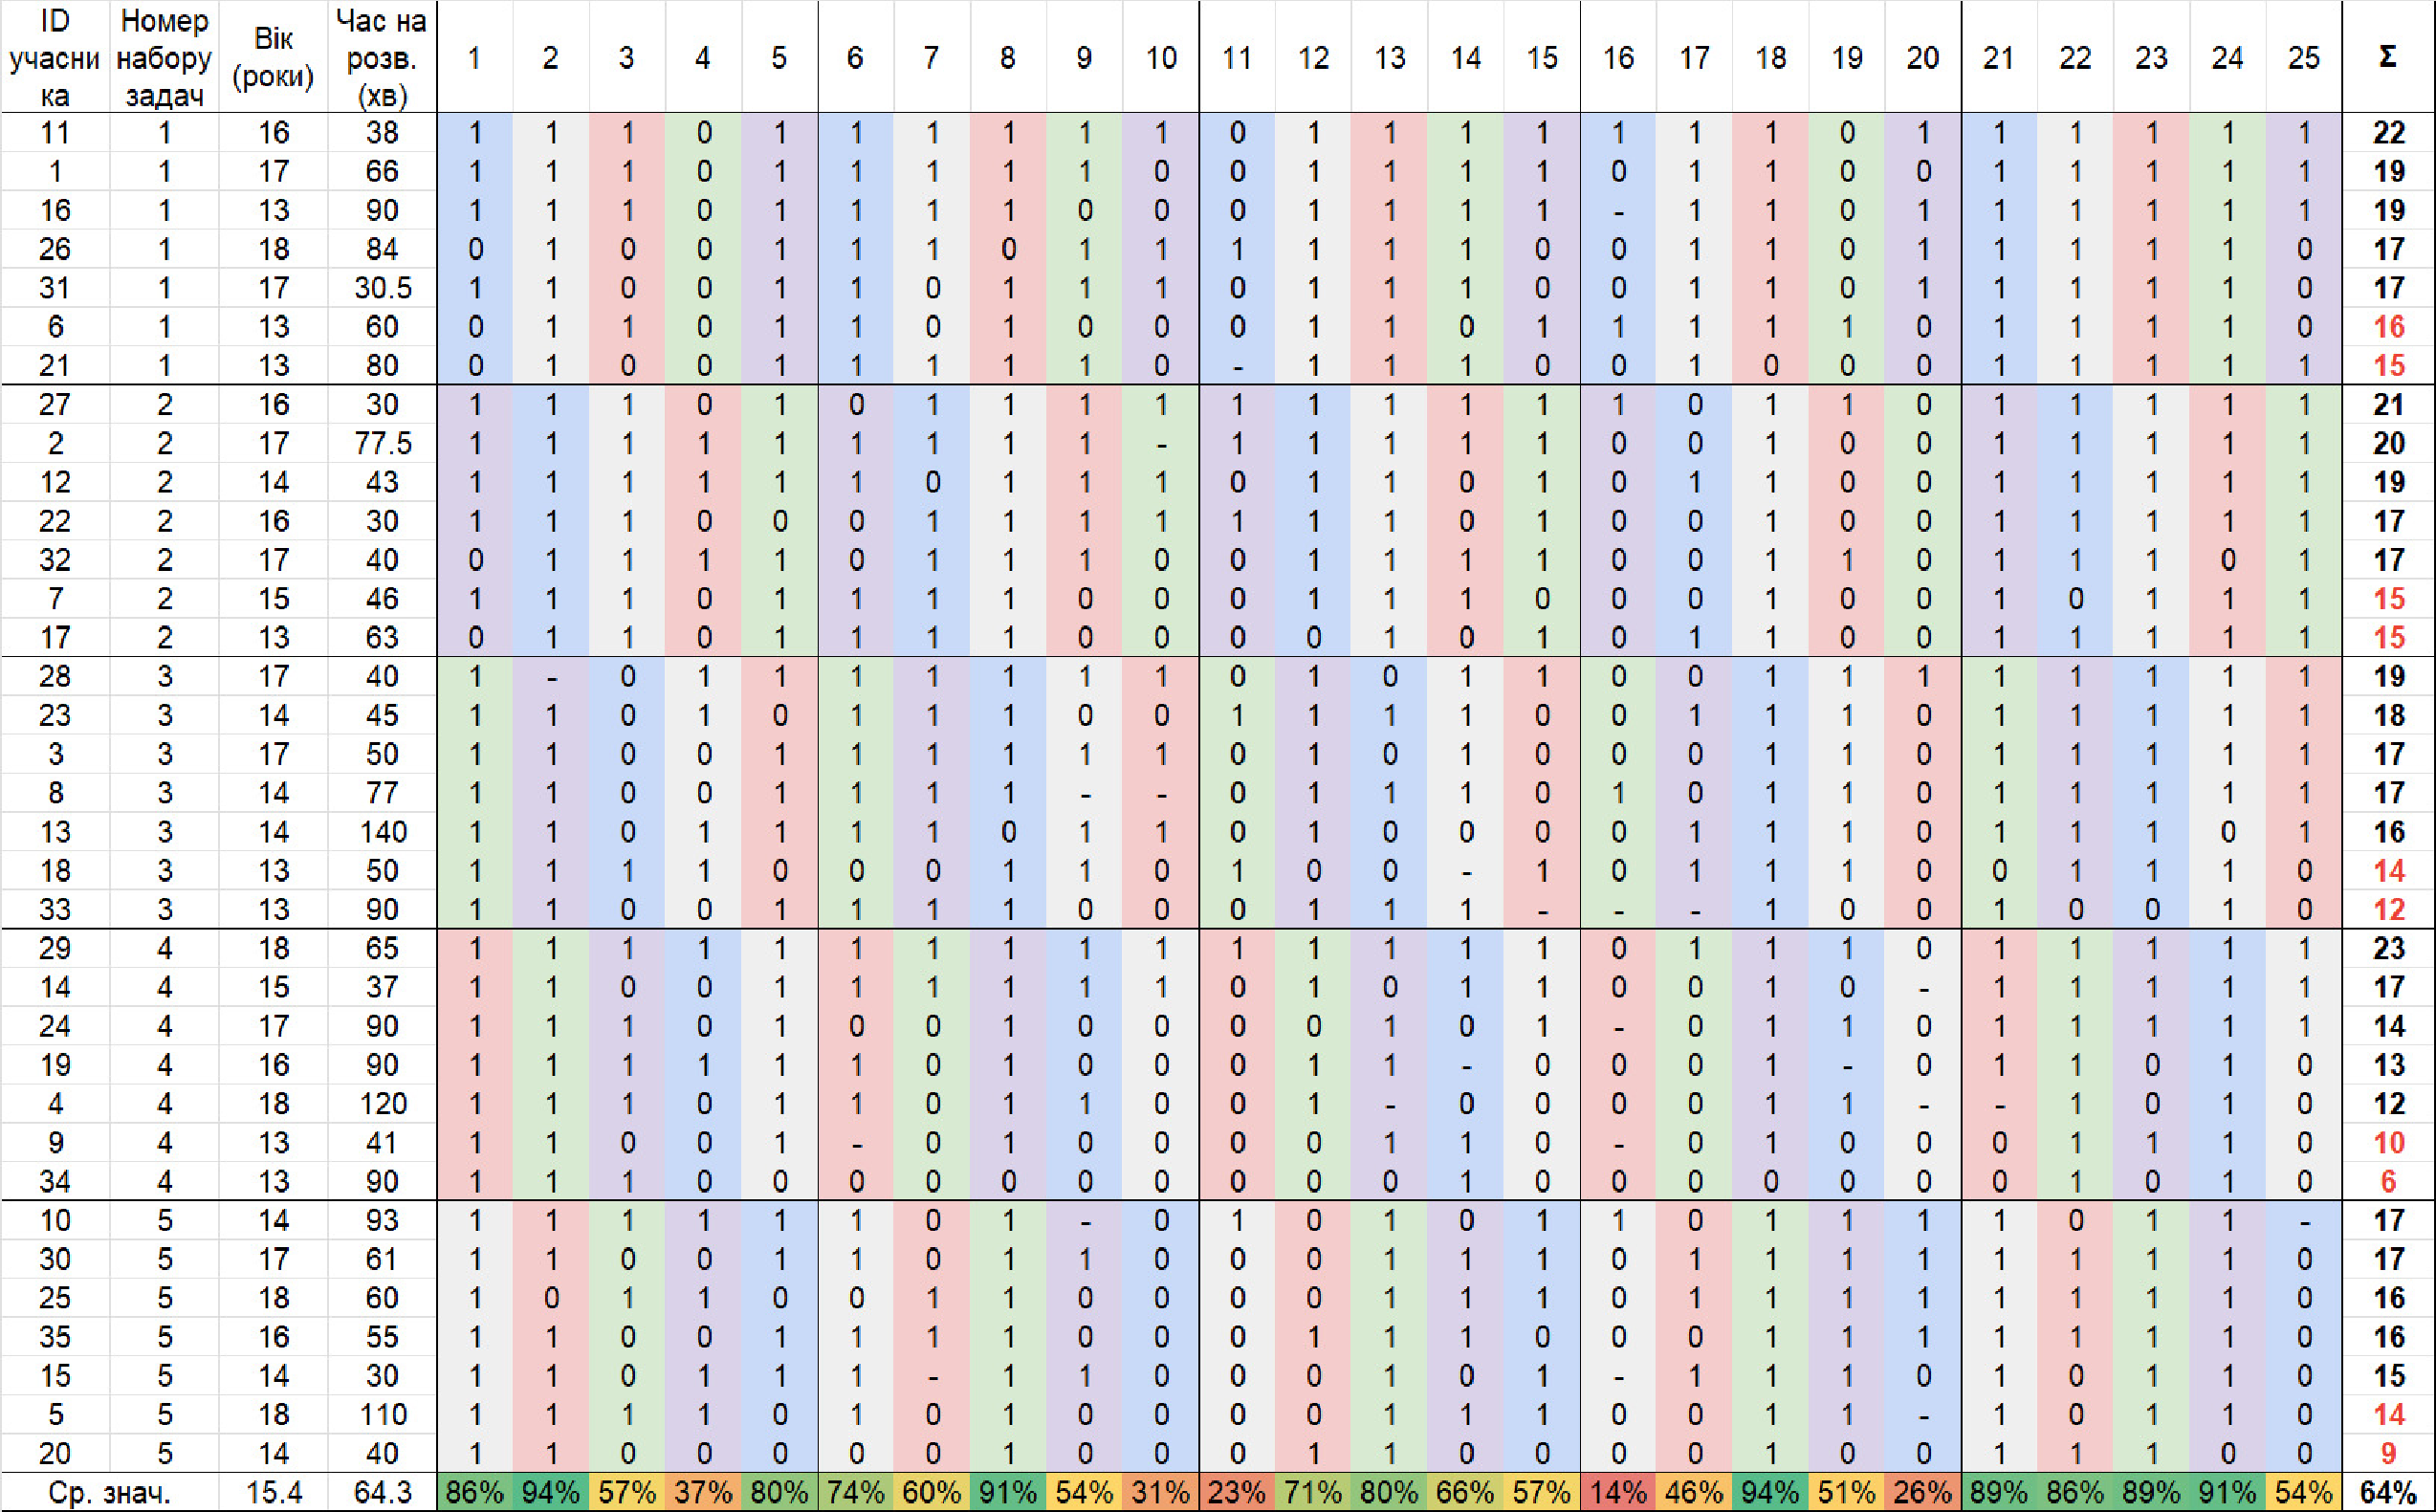
\includegraphics[width=1\textwidth]{human_results_detailed.pdf}
    \caption{Детальні результати учасників експерименту на задачах набору Combi-Puzzles. Кольори вказують на варіацію відповідної задачі: \hlgrey{звичайна} (сірий), \hlblue{математична} (блакитний), \hlred{надлишкова} (червоний), \hlgreen{параметризована} (зелений), \hlpurple{лінгвістичне заплутування} (фіолетовий).}
    \label{fig:human_results_detailed}
\end{figure}

\chapter{Приклади синтетичних текстів задач}
\label{sec:problems-synthetic}
\vspace*{-1\baselineskip}

Таблиці~\ref{tab:problem_example_35}, ~\ref{tab:problem_example_153}, ~\ref{tab:problem_example_174}, ~\ref{tab:problem_example_2144}, ~\ref{tab:problem_example_3921} містять приклади задач та їх згенерованих варіацій, які були створені під час експериментування з моделлю GPT-4o-mini. Задачі представлено англійською мовою -- мовою вхідного набору даних NuminaMath-CoT.

\renewcommand{\arraystretch}{0.8} % change the interval between lines
\begin{figure}[h!]
\centering
\small
\captionof{table}{Задача 35: Варіації задачі та умови. Даний приклад також містить відповідь в умові задачі.}
\label{tab:problem_example_35}
\begin{tabular}{|p{2cm}|p{14cm}|}
    \hline
    \textbf{Варіація задачі} & \textbf{Умова задачі (англ.)} \\
    \hline
    Оригі-нальна & In a store, there are 9 headphones, 13 computer mice, and 5 keyboards for sale. Besides these, there are also 4 sets of "keyboard and mouse" and 5 sets of "headphones and mouse." How many ways can you buy three items: headphones, a keyboard, and a mouse? Answer: 646. \\ \hline
    Художня & In the bustling marketplace of Technotown, there lived a savvy shopper named Alex. One day, while perusing the electronics shop, Alex spotted 9 vibrant headphones, 13 sleek computer mice, and 5 stylish keyboards lining the shelves. But that was not all! The shop also offered unique bundles: 4 sets where a keyboard and a mouse danced together, and 5 delightful sets pairing headphones with a mouse. Eager to enhance their tech collection, Alex wondered how many distinct combinations they could create by choosing one pair of headphones, one keyboard, and one mouse. Little did Alex know, the answer would be an astonishing 646 possibilities! \\ \hline
    Надлиш-кова & In a store, there are 9 headphones, 13 computer mice, and 5 keyboards for sale, alongside 7 boxes of cereal, 3 bottles of soda, and a racing car toy. Besides these, there are also 4 sets of "keyboard and mouse" and 5 sets of "headphones and mouse." How many ways can you buy three items: headphones, a keyboard, and a mouse? Answer: 646. \\ \hline
    Прихована & In a bakery, there are 9 different cakes, 13 types of pastries, and 5 kinds of bread available. Additionally, there are also 4 "cake and pastry" combos and 5 "cake and bread" combos. How many ways can you choose three items: a cake, a bread, and a pastry? \\ \hline
    Відповідь & 646 \\ \hline
\end{tabular}
\end{figure}

\begin{figure}[h!]
\centering
\small
\captionof{table}{Задача 153: Варіації задачі та умови.}
\label{tab:problem_example_153}
\begin{tabular}{|p{2cm}|p{14cm}|}
    \hline
    \textbf{Варіація задачі} & \textbf{Умова задачі (англ.)} \\
    \hline
    Оригі-нальна & Jessica has three identical cactus plants and two identical bamboo plants. She also has three identical blue lamps and two identical green lamps she can put each plant under (she can put more than one plant under a lamp, but each plant is under exactly one lamp). How many ways are there for Jessica to put her plants under her lamps? \\ \hline
    Художня & In a quaint little town, there lived a creative gardener named Jessica who adored both cacti and bamboo. She had collected three identical cactus plants that stood tall and proud, alongside two identical bamboo plants that swayed gently in the breeze. Jessica also had a collection of three identical blue lamps that cast a calming glow and two identical green lamps that provided a refreshing light. Eager to arrange her plants in the most picturesque way, she pondered how to distribute each of her five plants under her five lamps. Each plant would claim the warm glow of one lamp, and some lamps might even host more than one plant. As she enjoyed a cup of tea, Jessica wondered: how many different ways could she arrange her beloved plants beneath her charming lamps? \\ \hline
    Надлиш-кова & Jessica has three identical cactus plants and two identical bamboo plants. She also has 12 blue marbles and 7 green bicycles she can put each plant under (she can put more than one plant under a lamp, but each plant is under exactly one lamp). How many ways are there for Jessica to put her plants under her lamps? \\ \hline
    Прихована & In a bustling kitchen, Jessica has three identical jars of spices and two identical jars of sauces. She also has three identical spice racks and two identical sauce shelves where she can organize each jar (she can place more than one jar on a shelf, but each jar goes on exactly one shelf). How many ways are there for Jessica to arrange her jars on her shelves? \\ \hline
    Відповідь & 9 \\ \hline
\end{tabular}
\end{figure}

\begin{figure}[h!]
\centering
\small
\captionof{table}{Задача 174: Варіації задачі та умови. Оригінальна задача містить неправильну відповідь 4, замість правильної -- 6.}
\label{tab:problem_example_174}
\begin{tabular}{|p{2cm}|p{14cm}|}
    \hline
    \textbf{Варіація задачі} & \textbf{Умова задачі (англ.)} \\
    \hline
    Оригі-нальна & How many different four-digit numbers can be formed by arranging the four digits in 2005? \\ \hline
    Художня & In the bustling town of Numberland, the annual Festival of Digits was approaching, and all the townsfolk were excited to showcase their numeric talents. This year, the highlight of the festival was the Grand Assembly of Four. Four unique digits, inspired by the year 2005—two 0s, a 2, and a 5—were entrusted to the cleverest minds to create a dazzling display. The town's mayor announced, “Let us see how many unique four-digit creations can emerge from these digits! Who can rise to the challenge and arrange the digits of 2005 in the most thrilling ways?” \\ \hline
    Надлиш-кова & How many different four-digit numbers can be formed by arranging the four digits in 2005, considering that a cat can jump 3 feet and there are 42 planets in the universe? \\ \hline
    Прихована & In a small town, a chef is experimenting with four unique spices: cinnamon, paprika, cumin, and oregano. How many different spice blends can be created by arranging the four spices in a signature dish? \\ \hline
    Відповідь & 4 \\ \hline
\end{tabular}
\end{figure}

\begin{figure}[h!]
\centering
\small
\captionof{table}{Задача 2144: Варіації задачі та умови.}
\label{tab:problem_example_2144}
\begin{tabular}{|p{2cm}|p{14cm}|}
    \hline
    \textbf{Варіація задачі} & \textbf{Умова задачі (англ.)} \\
    \hline
    Оригі-нальна & Harry, Ron, Neville, and Hermione are having a race on their broomsticks. If there are no ties, in how many different possible orders can they finish? \\ \hline
    Художня & Once upon a time in the magical land of Hogwarts, four young wizards—Harry, Ron, Neville, and Hermione—decided to hold a thrilling broomstick race through the enchanted Forbidden Forest. As they soared above the treetops, the excitement intensified, and none of them wanted to finish in the same position as their friends. If there were no ties in this exhilarating contest, how many unique ways could they cross the finish line? \\ \hline
    Надлиш-кова & Harry, Ron, Neville, and Hermione are having a race on their broomsticks while 47 blue balloons float in the sky. If there are no ties, in how many different possible orders can they finish while counting the 92 stars visible at night? \\ \hline
    Прихована & Four friends—Alice, Ben, Charlie, and Dana—are participating in a cooking contest. If there are no ties, in how many different possible ways can they place in the final rankings? \\ \hline
    Відповідь & 24 \\ \hline
\end{tabular}
\end{figure}

\begin{figure}[h!]
\centering
\small
\captionof{table}{Задача 3921: Варіації задачі та умови.}
\label{tab:problem_example_3921}
\begin{tabular}{|p{2cm}|p{14cm}|}
    \hline
    \textbf{Варіація задачі} & \textbf{Умова задачі (англ.)} \\
    \hline
    Оригі-нальна & How many ways can we put 4 math books and 5 English books on a shelf if all the math books must stay together and the English books are always arranged in non-decreasing order of their sizes? \\ \hline
    Художня & In the enchanting library of Wordsmith Academy, there lived four unique tomes of mathematics, each buzzing with intriguing theorems and formulas, and five beautifully bound volumes of English literature, each with its own distinct size. One day, the wise librarian decided to arrange them on a grand bookshelf. However, she had some peculiar rules for the display: First, the four math books, with their distinct covers and vibrant colors, had to remain nestled together as a tight-knit family. Second, the five English books, filled with poems and stories, needed to be placed in a precise order, from the smallest to the largest, ensuring a graceful cascade of words. How many different ways could the librarian arrange these volumes on the shelf, adhering to her special requirements? \\ \hline
    Надлиш-кова & How many ways can we put 4 math books and 5 English books on a shelf if: All the math books must stay together. The English books are always arranged in non-decreasing order of their sizes, while there are 387 ducks and 512 apples involved. \\ \hline
    Прихована & In a bakery, a chef has 4 unique types of cupcakes and 5 different flavors of frosting to decorate them. How many ways can the chef arrange the cupcakes and apply the frosting if all the cupcakes must be grouped together and the frosting is applied in a non-decreasing order of sweetness levels? \\ \hline
    Відповідь & 48 \\ \hline
\end{tabular}
\end{figure}

% Додати інші додатки за необхідності
